\documentclass[pdf,aspectratio=169]{beamer}
\usepackage{xifthen}
\usepackage{listings}
\usepackage[ruled]{algorithm2e}
\usepackage{hhline}
\usepackage{appendixnumberbeamer}
\usepackage{forloop}

% Settings for listings package
\definecolor{mygreen}{rgb}{0,0.6,0}
\definecolor{mygray}{rgb}{0.5,0.5,0.5}
\definecolor{mymauve}{rgb}{0.58,0,0.82}
\definecolor{altblue}{rgb}{0.0,0.6,1.0}
\definecolor{lstbg}{gray}{0.9}

\lstdefinelanguage[firedrake]{python}[]{python}{%
  keywordstyle={[2]\color{red}},
   morekeywords={[2]UnitSquareMesh,interpolate,norm,offloading,MeshHierarchy,FunctionSpace,Function,TrialFunction,TestFunction,DirichletBC,SpatialCoordinate,Constant,solve},
  keywordstyle={[3]\color{orange}},
  morekeywords={[3]grad,dx,inner,pi,sin,cos,tan}
}
\lstdefinelanguage[highlighting]{python}[firedrake]{python}{
	moredelim=**[is][{\btHL[fill=red!30,draw=black,thin]}]{`mesh*}{`},
	moredelim=**[is][{\btHL[fill=orange!30,draw=black,thin]}]{`fs*}{`},
	moredelim=**[is][{\btHL[fill=mygreen!30,draw=black,thin]}]{`bcs*}{`},
	moredelim=**[is][{\btHL[fill=blue!30,draw=black,thin]}]{`rhs*}{`},
	moredelim=**[is][{\btHL[fill=violet!30,draw=black,thin]}]{`bilf*}{`}
}

\graphicspath{{./figures/}}

\mode<presentation>{
    \usetheme{firedrake}
	\usecolortheme{firedrake}
}

% Awkward widebar thing... (instead of mathabx)
\makeatletter
\newcommand*\rel@kern[1]{\kern#1\dimexpr\macc@kerna}
\newcommand*\widebar[1]{%
  \begingroup
  \def\mathaccent##1##2{%
    \rel@kern{0.8}%
    \overline{\rel@kern{-0.8}\macc@nucleus\rel@kern{0.2}}%
    \rel@kern{-0.2}%
  }%
  \macc@depth\@ne
  \let\math@bgroup\@empty \let\math@egroup\macc@set@skewchar
  \mathsurround\z@ \frozen@everymath{\mathgroup\macc@group\relax}%
  \macc@set@skewchar\relax
  \let\mathaccentV\macc@nested@a
  \macc@nested@a\relax111{#1}%
  \endgroup
}
\makeatother

% Some tikz magic
\usepackage{tikz}
\usetikzlibrary{arrows}

% Define how TiKZ will draw the nodes
\tikzset{term/.style={draw=none,fill=none,rectangle,inner sep=0pt,anchor=base}}
\tikzstyle{every picture}+=[remember picture]
\everymath{\displaystyle}

\makeatletter

% Designate a term in a math environment to point to
% Syntax: \mathterm[node label]{some math}
\newcommand\mathterm[2][]{%
  \@ifnextchar[{\@mathtermopts{#1}{#2}}{\@mathtermnoopts{#1}{#2}}}
\def\@mathtermnoopts#1#2{%
  \tikz [baseline] { \node [term] (#1) {$#2$}; }}
\def\@mathtermopts#1#2[#3]{%
  \tikz [baseline] { \node [rectangle,inner sep=2pt,rounded corners=2pt,anchor=base,,#3] (#1) {$#2$}; }}

\newcommand\textterm[2][]{%
  \@ifnextchar[{\@texttermopts{#1}{#2}}{\@texttermnoopts{#1}{#2}}}
\def\@texttermnoopts#1#2{%
  \tikz [baseline] { \node [term] (#1) {#2}; }}
\def\@texttermopts#1#2[#3]{%
  \tikz [baseline] { \node [rectangle,inner sep=2pt,rounded corners=2pt,anchor=base,,#3] (#1) {#2}; }}

% A command to draw an arrow from the current position to a labelled math term
% Default color=black, default arrow head=stealth
% Syntax: \indicate[color]{term to point to}[path options]
\newcommand\indicate[2][black]{%
  \tikz [baseline] \node [inner sep=0pt,anchor=base] (i#2) {\vphantom|};
  \@ifnextchar[{\@indicateopts{#1}{#2}}{\@indicatenoopts{#1}{#2}}}
\def\@indicatenoopts#1#2{%
  {\color{#1} \tikz[overlay] \path[line width=1pt,draw=#1,-stealth] (i#2) edge (#2);}}
\def\@indicateopts#1#2[#3]{%
  {\color{#1} \tikz[overlay] \path[line width=1pt,draw=#1,-stealth] (i#2) [#3] edge (#2);}}

\newenvironment{btHighlight}[1][]
{\begingroup\tikzset{bt@Highlight@par/.style={#1}}\begin{lrbox}{\@tempboxa}}
{\end{lrbox}\bt@HL@box[bt@Highlight@par]{\@tempboxa}\endgroup}

\newcommand\btHL[1][]{%
  \begin{btHighlight}[#1]\bgroup\aftergroup\bt@HL@endenv%
}
\def\bt@HL@endenv{%
  \end{btHighlight}%
  \egroup
}
\newcommand{\bt@HL@box}[2][]{%
  \tikz[#1]{%
    \pgfpathrectangle{\pgfpoint{1pt}{0pt}}{\pgfpoint{\wd #2}{\ht #2}}%
    \pgfusepath{use as bounding box}%
    \node[anchor=base west, fill=orange!30,outer sep=0pt,inner xsep=1pt, inner ysep=0pt, rounded corners=2pt, minimum height=\ht\strutbox+1pt,#1]{\raisebox{1pt}{\strut}\strut\usebox{#2}};
  }%
}
\makeatother

%%%%% BEGIN lstlinebgrd highlighting
% Bug in lstlinebgrd
\makeatletter
\let\old@lstKV@SwitchCases\lstKV@SwitchCases
\def\lstKV@SwitchCases#1#2#3{}
\makeatother
\usepackage{lstlinebgrd}
\makeatletter
\let\lstKV@SwitchCases\old@lstKV@SwitchCases

\lst@Key{numbers}{none}{%
    \def\lst@PlaceNumber{\lst@linebgrd}%
    \lstKV@SwitchCases{#1}%
    {none:\\%
     left:\def\lst@PlaceNumber{\llap{\normalfont
                \lst@numberstyle{\thelstnumber}\kern\lst@numbersep}\lst@linebgrd}\\%
     right:\def\lst@PlaceNumber{\rlap{\normalfont
                \kern\linewidth \kern\lst@numbersep
                \lst@numberstyle{\thelstnumber}}\lst@linebgrd}%
    }{\PackageError{Listings}{Numbers #1 unknown}\@ehc}}
%%%%%%%%%%%%%%%%%%%%%%%%%%%%%%%%%%%%%%%%%%%%%%%%%%%%%%%%%%%%%%%%%%%%%%%%%%%%%%
%
% \btIfInRange{number}{range list}{TRUE}{FALSE}
%
% Test in int number <number> is element of a (comma separated) list of ranges
% (such as: {1,3-5,7,10-12,14}) and processes <TRUE> or <FALSE> respectively
\newcount\bt@rangea
\newcount\bt@rangeb

\newcommand\btIfInRange[2]{%
    \global\let\bt@inrange\@secondoftwo%
    \edef\bt@rangelist{#2}%
    \foreach \range in \bt@rangelist {%
        \afterassignment\bt@getrangeb%
        \bt@rangea=0\range\relax%
        \pgfmathtruncatemacro\result{ ( #1 >= \bt@rangea) && (#1 <= \bt@rangeb) }%
        \ifnum\result=1\relax%
            \breakforeach%
            \global\let\bt@inrange\@firstoftwo%
        \fi%
    }%
    \bt@inrange%
}
\newcommand\bt@getrangeb{%
    \@ifnextchar\relax%
        {\bt@rangeb=\bt@rangea}%
        {\@getrangeb}%
}
\def\@getrangeb-#1\relax{%
    \ifx\relax#1\relax%
        \bt@rangeb=100000%   \maxdimen is too large for pgfmath
    \else%
        \bt@rangeb=#1\relax%
    \fi%
}

%%%%%%%%%%%%%%%%%%%%%%%%%%%%%%%%%%%%%%%%%%%%%%%%%%%%%%%%%%%%%%%%%%%%%%%%%%%%%%
%
% \btLstHL<overlay spec>{range list}
%
% TODO BUG: \btLstHL commands can not yet be accumulated if more than one overlay spec match.
%
\newcommand<>{\btLstHL}[1]{%
  \only#2{\btIfInRange{\value{lstnumber}}{#1}{\color{black!30}\def\lst@linebgrdcmd{\color@block}}{\def\lst@linebgrdcmd####1####2####3{}}}%
}%
\makeatother
%%%%% END lstlinebgrd highlighting

\lstset{
  backgroundcolor=\color{lstbg},
  % choose the background color; you must add \usepackage{color} or \usepackage{xcolor}
  basicstyle=\tiny\ttfamily,
  % the size of the fonts that are used for the code
  breakatwhitespace=true,
  % sets if automatic breaks should only happen at whitespace
  breaklines=true,
  % sets automatic line breaking
  captionpos=b,
  % sets the caption-position to bottom
  commentstyle=\color{mygreen},
  % comment style
  deletekeywords={},
  % if you want to delete keywords from the given language
  escapeinside={\#*}{*},
  % if you want to add LaTeX within your code
  extendedchars=true,
  % lets you use non-ASCII characters; for 8-bits encodings only, does not work with UTF-8
  frame=single,
  % adds a frame around the code
  keepspaces=true,
  % keeps spaces in text, useful for keeping indentation of code (possibly needs columns=flexible)
  keywordstyle=\color{blue},
  % keyword style
  %language=c++,
  % the language of the code
  otherkeywords={},
  % if you want to add more keywords to the set
  numbers=left,
  % where to put the line-numbers; possible values are (none, left, right)
  numbersep=5pt,
  % how far the line-numbers are from the code
  numberstyle=\tiny\color{mygray},
  % the style that is used for the line-numbers
  rulecolor=\color{black},
  % if not set, the frame-color may be changed on line-breaks within not-black text (e.g. comments (green here))
  showspaces=false,
  % show spaces everywhere adding particular underscores; it overrides 'showstringspaces'
  showstringspaces=false,
  % underline spaces within strings only
  showtabs=false,
  % show tabs within strings adding particular underscores
  stepnumber=1,
  % the step between two line-numbers. If it's 1, each line will be numbered
  stringstyle=\color{mymauve},
  % string literal style
  tabsize=4,
  % sets default tabsize to 4 spaces
  title=\lstname,
  % show the filename of files included with \lstinputlisting; also try caption instead of title
  linebackgroundsep=3pt,linebackgroundwidth={\dimexpr\linewidth+6pt\relax}
  %adjustments for lstlinebgrd highlighting
}

\newcommand{\citehere}[1]{{\footnotesize[#1]}}

\newcounter{nrank}

\title[]{On the Road to GPUs\\
\small SysGenX Meetup}
\author[JB,PF,DH]{David Ham \and Patrick Farrell \and \textbf{Jack Betteridge}}
\date[27/9/2022]{27${}^\text{th}$ September 2022}

\begin{document}
\maketitle

%%%%%%%%%%%%%%%%%%%%%%%%%%%%%%%%%%%%%%%%%%%%%%%%%%%%%%%%%%%%%%%%%%%%%%%%%%%%%%%%
\begin{frame}{Update}
What have we been working on?
\begin{itemize}
	\item Spack installer
	\item Petsc4py garbage collector
	\item Scaling software components on ARCHER2
	\item The road to GPUs!
\end{itemize}

\end{frame}

%%%%%%%%%%%%%%%%%%%%%%%%%%%%%%%%%%%%%%%%%%%%%%%%%%%%%%%%%%%%%%%%%%%%%%%%%%%%%%%%
\begin{frame}
    Didn't most of this get presented last time!?
	
\includegraphics[width=0.8\textwidth]{well_yes.jpg}
\end{frame}

%%%%%%%%%%%%%%%%%%%%%%%%%%%%%%%%%%%%%%%%%%%%%%%%%%%%%%%%%%%%%%%%%%%%%%%%%%%%%%%%
\begin{frame}{Spack}
    \begin{figure}
	    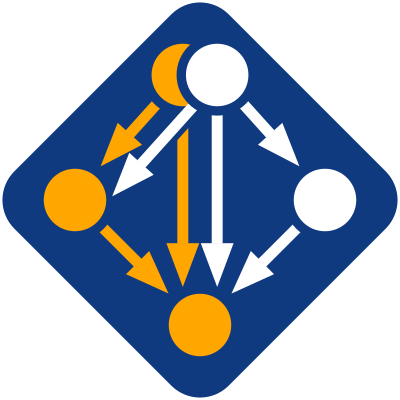
\includegraphics[width=0.1\textwidth]{spack-logo.png}
    \end{figure}
    
	This is a moving target:
	\begin{itemize}
	\item Spack is still ``alpha'' software, but widely used on HPC\uncover<2->{, problematic!}
	\item Package repo included in Spack code repo\uncover<3->{, problematic!}
	\item All dependencies have a habit of changing/updating\uncover<4->{, frustrating!}
	\item Support on ARCHER2 soon...
	
	\centering{\uncover<5->{...but won't be enough}}
\end{itemize}

\end{frame}

%%%%%%%%%%%%%%%%%%%%%%%%%%%%%%%%%%%%%%%%%%%%%%%%%%%%%%%%%%%%%%%%%%%%%%%%%%%%%%%%
\begin{frame}{Garbage Collector}
	Work is done! But, not merged into PETSc (yet...)
	
	We already have users:
	\begin{itemize}\vspace{-2pt}\setlength{\itemsep}{0em}
	\item Checkpointing
	\item Deflation
	\item Julia
    \end{itemize}

	Still not merged
	\begin{itemize}\vspace{-2pt}\setlength{\itemsep}{0em}
	\item Changes to base PETSc objects/routines.
	\item Needs to be right, but also easy to use.
	\item Need to make sure we're on same page as PETSc devs.
    \end{itemize}
\end{frame}

%%%%%%%%%%%%%%%%%%%%%%%%%%%%%%%%%%%%%%%%%%%%%%%%%%%%%%%%%%%%%%%%%%%%%%%%%%%%%%%%
\begin{frame}{ARCHER2}
\begin{figure}
    \centering
    
\includegraphics[width=0.3\textwidth]{archer2_logo.png}
\end{figure}
In conversation with EPCC/ARCHER2 support:
\begin{itemize}
	\item Spack coming to ARCHER2 soon
    \item Singularity is currently supported
    \begin{itemize}
	    \item Great for end users who don't need to develop internals
        \item Good for Capability demonstrating applications too?
    \end{itemize}
    \item Spindle now being considered
    \begin{itemize}
	    \item Help Python init on massive node counts
	    \item Not User/Spack installable
    \end{itemize}
    \item There \emph{will} be GPUs!
\end{itemize}

\end{frame}

%%%%%%%%%%%%%%%%%%%%%%%%%%%%%%%%%%%%%%%%%%%%%%%%%%%%%%%%%%%%%%%%%%%%%%%%%%%%%%%%
\begin{frame}{GPU}
\begin{columns}
\begin{column}[T]{0.49\textwidth}
    Target the GPU as an offload device:
    \begin{itemize}
	\item Use OpenCL framework (CUDA future?)
	\item Use a context manager to control offloading:\\
	One form assembly(+matfree)/\\Solvers/\\(Matrix assembly)
    \end{itemize}
    
    Follow dependencies:
    \begin{itemize}
	\item loo.py
	\item PETSc
    \end{itemize}
    
    \hspace{3em} Follow the hardware:\\
    \hspace{4em} Not all GPUs are NVidia!
\end{column}
\begin{column}[T]{0.49\textwidth}
    \begin{figure}
        \centering
	    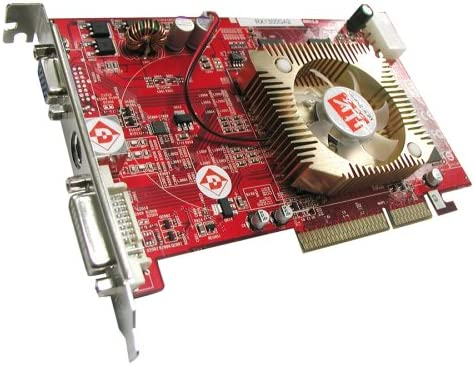
\includegraphics[width=0.9\textwidth]{gpu3.jpg}
	\end{figure}
\end{column}
\end{columns}
\end{frame}

\begin{frame}[fragile]{GPU}
\begin{columns}
\begin{column}[T]{0.49\textwidth}
\begin{lstlisting}[language={[firedrake]python},linebackgroundcolor={\btLstHL{15,16,22,23}},caption={Example GPU utilisation}]
mesh = UnitSquareMesh(32, 32)
V = FunctionSpace(mesh, "CG", 1)
u = TrialFunction(V)
v = TestFunction(V)
x, y = SpatialCoordinate(mesh)

a = (inner(grad(u), grad(v)) + inner(u, v)) * dx
f = Function(V)
f.interpolate((1+8*pi*pi)*cos(x*pi*2)*cos(y*pi*2))
L = inner(f, v) * dx
fem_soln = Function(V)
sp = {"mat_type": "matfree",
      "ksp_monitor_true_residual": None,
      "ksp_converged_reason": None}
with offloading():
    solve(a == L, fem_soln, solver_parameters=sp)

f.interpolate(cos(x*pi*2)*cos(y*pi*2))

assert norm(fem_soln-f) < 1e-2

with offloading():
    assert norm(fem_soln-f) < 1e-2
\end{lstlisting}
\end{column}
\begin{column}[T]{0.49\textwidth}
    Do not want user code to be significantly different.
    
    \vspace{0.5em}
    Manage offloading to accelerators through Python context managers (highlighted).
    
    \vspace{0.5em}
    Slightly more than vapourware:
    \begin{itemize}
	\item Firedrake branch with functionality
	\item Currently only tested for CPU \emph{on CI}
	\item Raises questions about robust CI
    \end{itemize}
    
    Want to maintain portability between user machine and HPC.
\end{column}
\end{columns}
\end{frame}

\begin{frame}{Code generation}
	\begin{center}Firedrake $\rightarrow$ PyOP2 $\rightarrow$ loo.py\end{center}
	
	Initially targeting OpenCL:
	\begin{itemize}\vspace{-2pt}\setlength{\itemsep}{0em}
	\item Already partially supported in loo.py
	\item Working with Kaushik Kulkarni (loo.py) to get everything we need integrated
    \end{itemize}
	
	PyOP2 won't use ``backends'':
	\begin{itemize}\vspace{-2pt}\setlength{\itemsep}{0em}
	\item Rather have a ``mirrored array''
	\item Will use "backend mixins" where necessary
	\item Ensure host $\leftrightarrow$ device copies minimised
	\item Some concern over client driver support
\end{itemize}
    Will be incorperated into a wider refactoring of PyOP2 (Connor Ward)
	
	\hspace{3em}Later consider targeting CUDA
	
	
\end{frame}

\begin{frame}{PETSc}
\vspace{-2em}
\begin{figure}
    \centering
    
\includegraphics[width=0.3\textwidth]{petsc.png}
\end{figure}
\vspace{-2em}
Supports OpenCL using the ViennaCL library:
\begin{itemize}
	\item NVidia, AMD and Intel targets${}^\dagger$ \uncover<3->{\hspace{2em}-requires working client driver!}
	\item Currently supported in loo.py
\end{itemize}

\begin{columns}
\begin{column}[T]{0.49\textwidth}
    PETSc also supports:
    \begin{itemize}
	\item CUDA* (cuBLAS/cuSparse),
	\item HIP* (ROCm),
	\item Kokkos, 
	\item Future work: SYCL** (MKL)
    \end{itemize}
\end{column}
\begin{column}[T]{0.49\textwidth}
    \uncover<2->{Caveats:
    \begin{itemize}
	\item NVidia only
	\item AMD only
	\item Not currently supported
	\item ???
    \end{itemize}
    }
\end{column}
\end{columns}
 
\end{frame}

\begin{frame}{GPGPU resources}
Still in getting started phase.

Recently higlighted was lack of available training and resources.

Happy to hear recommendations about:
\begin{itemize}
	\item Courses,
	\item Tutorials,
	\item Materials,
\end{itemize}
for GPGPU programming.
\end{frame}

\end{document}
